\documentclass{article}

% if you need to pass options to natbib, use, e.g.:
% \PassOptionsToPackage{numbers, compress}{natbib}
% before loading nips_2018

% ready for submission
\usepackage{nips_2018}

% to compile a preprint version, e.g., for submission to arXiv, add
% add the [preprint] option:
% \usepackage[preprint]{nips_2018}

% to compile a camera-ready version, add the [final] option, e.g.:
% \usepackage[final]{nips_2018}

% to avoid loading the natbib package, add option nonatbib:
% \usepackage[nonatbib]{nips_2018}

\usepackage[utf8]{inputenc} % allow utf-8 input
\usepackage[T1]{fontenc}    % use 8-bit T1 fonts
\usepackage{hyperref}       % hyperlinks
\usepackage{url}            % simple URL typesetting
\usepackage{booktabs}       % professional-quality tables
\usepackage{amsfonts}       % blackboard math symbols
\usepackage{amssymb}
\usepackage{amsmath}
\usepackage{nicefrac}       % compact symbols for 1/2, etc.
\usepackage{microtype}      % microtypography
\usepackage{graphicx}
\usepackage{xcolor}
\usepackage{tikz}
\usetikzlibrary{matrix,backgrounds}
\usetikzlibrary{positioning}
\usetikzlibrary{shapes,arrows}
\usetikzlibrary{decorations.pathreplacing,angles,quotes}


\tikzstyle{block} = [rectangle, draw, fill=red!20!blue!10,
    text width=5em, text centered, rounded corners, minimum height=4em]
\tikzstyle{netnode} = [circle, draw, very thick, inner sep=0pt, minimum size=0.5cm]
\tikzstyle{relunode} = [rectangle, draw, very thick, inner sep=0pt, minimum size=0.5cm]

\tikzstyle{line} = [draw, line width=1.5pt, -latex']

\newcommand{\R}{\mathbb{R}}


\title{Generalization \& Transfer}

% The \author macro works with any number of authors. There are two
% commands used to separate the names and addresses of multiple
% authors: \And and \AND.
%
% Using \And between authors leaves it to LaTeX to determine where to
% break the lines. Using \AND forces a line break at that point. So,
% if LaTeX puts 3 of 4 authors names on the first line, and the last
% on the second line, try using \AND instead of \And before the third
% author name.

\author{
  Andrew K. Lampinen\thanks{\url{http://web.stanford.edu/~lampinen/}} \\
  Department of Psychology\\
  Stanford University \\
  Stanford, CA 94305 \\
  \texttt{lampinen@stanford.edu} \\
  \And
  James L. McClelland \\
  Department of Psychology\\
  Stanford University \\
  Stanford, CA 94305 \\
  \texttt{mcclelland@stanford.edu} \\
  \And
  Surya Ganguli \\
  Department of Applied Physics\\
  Stanford University \\
  Stanford, CA 94305 \\
  \texttt{sganguli@stanford.edu} \\
}

\begin{document}
% \nipsfinalcopy is no longer used

\maketitle

\begin{abstract}
\end{abstract}

\section{Introduction}

The rise to dominance of deep learning models in recent years has been driven by their ability to provide strong generalization. This underlies the success of deep learning systems in diverse tasks such as image classification \cite{}. However we lack theoretical understanding of this generalization -- classic theoretical bounds on generalization (VC dimension, etc.) are overly pessimistic when applied to neural networks \citep{Zhang2016, Advani2017}. \par 
Furthermore, multi-task learning can improve generalization even further \cite[e.g.]{Dong2015,Rusu2015}. Even a small amount of learning on distinct but related tasks has been shown to improve performance. For example, training a natural language translation system on image captioning and autoencoding improves translation performance \citep{Luong2016}. Learning on numerous language translation pairs can even give generalization without further training to unseen language pairs \citep{Johnson2016a}. That is, generalization seems to be improved by learning multiple tasks that share some underlying structure. In prior work, we have suggested that this cross-task learning may be key to human generalization abilities \citep{Hansen2017, Lampinen2017a}. How can we quantify the relationship between shared structure in multiple tasks and generalization performance? \par 
In this paper, we explore these issues within linear neural networks. Linear neural networks have proven a fruitful ground for theoretical work, and are often close enough to non-linear networks that theoretical results approximately generalize, or at least provide useful intuitions \cite[e.g.]{Saxe2013, Advani2017}. We offer new theoretical results exploring generalization and multi-task learning. \par
\subsection{Prior work}
Prior work on generalization has focused on single outputs \cite[e.g.]{Advani2017}. However, most of the powerful recent results from neural networks have come from settings with multiple outputs, either multiple related tasks, or more complex output spaces (language models outputting word vectors or sequences of word vectors, GANs outputting images \cite{Goodfellow2014}, reinforcement learning systems outputting policies or values \cite{Mnih2015, Silver2016}, etc.). Our work addresses how the structure shared between multiple outputs affects generalization with noisy training data. \par 
\section{General theoretical setting}
We consider the general setting where there is some true linear function \(f: \R^N \rightarrow \R^K\) to be learned, which can be thought of as a ``teacher'' linear neural network with \(N\) inputs and \(K\) outputs. We consider the task of a ``student'' neural network with an identical architecture to the teacher, which learns by training on a dataset generated from the teacher, but with IID noise added to every output node on each training example. This noise is fixed across training, so that the student network will have a signal to overfit to. This reflects the fact that we generally train deep learning systems on a large but fixed sample from the true data distribution. We evaluate generalization by how closely the function parameterized by the student (\(g\)) matches the ground-truth teacher function (\(f\)). In other words, we evaluate generaliation based on how well the network is able to overcome the noise on the training data and learn the underlying function, by evaluating test error on noiseless data. \par
We use one-hot inputs and explore how structure in the input-output correlation of the true function \(f\), the strength of the noise added to the data, and the length of training influence the generalization performance of the student network. 

\begin{figure}
\centering
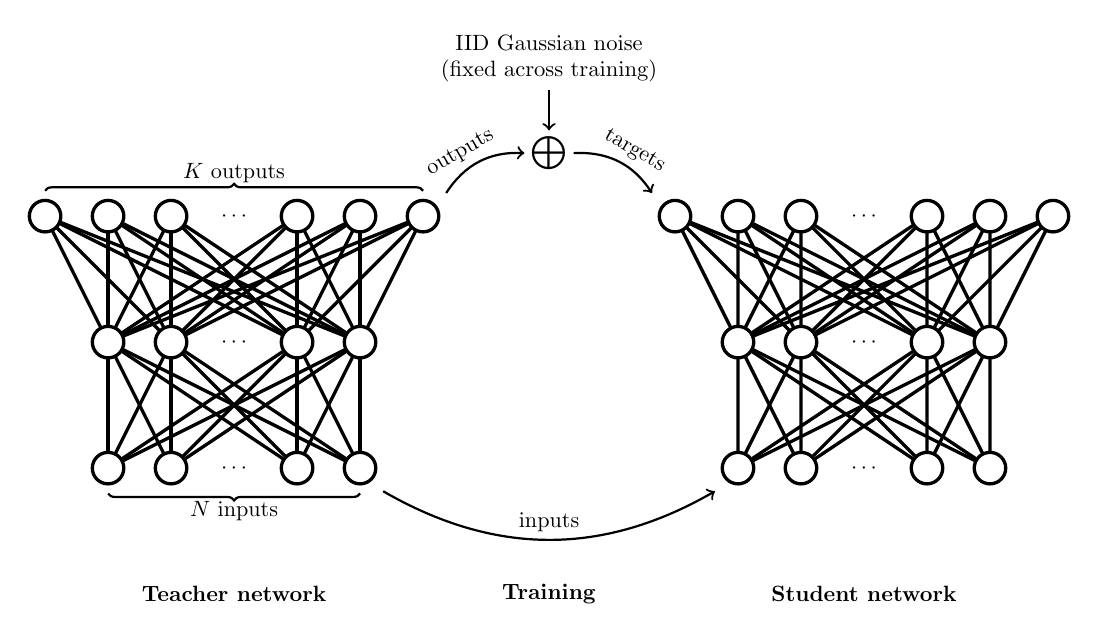
\begin{tikzpicture}[auto, scale=0.8, every node/.style={scale=0.8}]
%%%% teacher
% input layer

\node [netnode] at (-2,0) (i1) {};
\node [netnode] at (-1,0) (i2) {};
\node at (0, 0) (id) {\(\cdots\)};
\node [netnode] at (1,0) (i3) {};
\node [netnode] at (2,0) (i4) {};
\draw[decoration={brace,mirror, raise=3pt},decorate, thick] (i1.south) -- node[below = 0.1] {$N$ inputs} (i4.south);


% hidden layer
\node [netnode] at (-2,2) (h1) {};
\node [netnode] at (-1,2) (h2) {};
\node at (0,2) (hd) {\(\cdots\)};
\node [netnode] at (1,2) (h3) {};
\node [netnode] at (2,2) (h4) {};

% output layer
\node [netnode] at (-3,4) (o0) {};
\node [netnode] at (-2,4) (o1) {};
\node [netnode] at (-1,4) (o2) {};
\node at (0,4) (od) {\(\cdots\)};
\node [netnode] at (1,4) (o3) {};
\node [netnode] at (2,4) (o4) {};
\node [netnode] at (3,4) (o5) {};
\draw[decoration={brace,raise=3pt},decorate, thick] (o0.north) -- node[above = 0.1] {$K$ outputs} (o5.north);

\node at (0, -2) (teach) {\textbf{Teacher network}};

% input -> hidden
\path [draw, very thick] (i1) to (h1);
\path [draw, very thick] (i1) to (h2);
\path [draw, very thick] (i1) to (h3);
\path [draw, very thick] (i1) to (h4);
\path [draw, very thick] (i2) to (h1);
\path [draw, very thick] (i2) to (h2);
\path [draw, very thick] (i2) to (h3);
\path [draw, very thick] (i2) to (h4);
\path [draw, very thick] (i3) to (h1);
\path [draw, very thick] (i3) to (h2);
\path [draw, very thick] (i3) to (h3);
\path [draw, very thick] (i3) to (h4);
\path [draw, very thick] (i4) to (h1);
\path [draw, very thick] (i4) to (h2);
\path [draw, very thick] (i4) to (h3);
\path [draw, very thick] (i4) to (h4);

% hidden -> output
\path [draw, very thick] (h1) to (o1);
\path [draw, very thick] (h1) to (o2);
\path [draw, very thick] (h1) to (o3);
\path [draw, very thick] (h1) to (o4);
\path [draw, very thick] (h2) to (o1);
\path [draw, very thick] (h2) to (o2);
\path [draw, very thick] (h2) to (o3);
\path [draw, very thick] (h2) to (o4);
\path [draw, very thick] (h3) to (o1);
\path [draw, very thick] (h3) to (o2);
\path [draw, very thick] (h3) to (o3);
\path [draw, very thick] (h3) to (o4);
\path [draw, very thick] (h4) to (o1);
\path [draw, very thick] (h4) to (o2);
\path [draw, very thick] (h4) to (o3);
\path [draw, very thick] (h4) to (o4);

\path [draw, very thick] (h1) to (o0);
\path [draw, very thick] (h2) to (o0);
\path [draw, very thick] (h3) to (o0);
\path [draw, very thick] (h4) to (o0);
\path [draw, very thick] (h1) to (o5);
\path [draw, very thick] (h2) to (o5);
\path [draw, very thick] (h3) to (o5);
\path [draw, very thick] (h4) to (o5);

%%%%% student
\node at (10, -2) (stud) {\textbf{Student network}};
% input layer

\node [netnode] at (8,0) (si1) {};
\node [netnode] at (9,0) (si2) {};
\node at (10, 0) (sid) {\(\cdots\)};
\node [netnode] at (11,0) (si3) {};
\node [netnode] at (12,0) (si4) {};

% hidden layer
\node [netnode] at (8,2) (sh1) {};
\node [netnode] at (9,2) (sh2) {};
\node at (10,2) (shd) {\(\cdots\)};
\node [netnode] at (11,2) (sh3) {};
\node [netnode] at (12,2) (sh4) {};

% output layer
\node [netnode] at (7,4) (so0) {};
\node [netnode] at (8,4) (so1) {};
\node [netnode] at (9,4) (so2) {};
\node at (10,4) (sod) {\(\cdots\)};
\node [netnode] at (11,4) (so3) {};
\node [netnode] at (12,4) (so4) {};
\node [netnode] at (13,4) (so5) {};

% input -> hidden
\path [draw, very thick] (si1) to (sh1);
\path [draw, very thick] (si1) to (sh2);
\path [draw, very thick] (si1) to (sh3);
\path [draw, very thick] (si1) to (sh4);
\path [draw, very thick] (si2) to (sh1);
\path [draw, very thick] (si2) to (sh2);
\path [draw, very thick] (si2) to (sh3);
\path [draw, very thick] (si2) to (sh4);
\path [draw, very thick] (si3) to (sh1);
\path [draw, very thick] (si3) to (sh2);
\path [draw, very thick] (si3) to (sh3);
\path [draw, very thick] (si3) to (sh4);
\path [draw, very thick] (si4) to (sh1);
\path [draw, very thick] (si4) to (sh2);
\path [draw, very thick] (si4) to (sh3);
\path [draw, very thick] (si4) to (sh4);

% hidden -> output
\path [draw, very thick] (sh1) to (so1);
\path [draw, very thick] (sh1) to (so2);
\path [draw, very thick] (sh1) to (so3);
\path [draw, very thick] (sh1) to (so4);
\path [draw, very thick] (sh2) to (so1);
\path [draw, very thick] (sh2) to (so2);
\path [draw, very thick] (sh2) to (so3);
\path [draw, very thick] (sh2) to (so4);
\path [draw, very thick] (sh3) to (so1);
\path [draw, very thick] (sh3) to (so2);
\path [draw, very thick] (sh3) to (so3);
\path [draw, very thick] (sh3) to (so4);
\path [draw, very thick] (sh4) to (so1);
\path [draw, very thick] (sh4) to (so2);
\path [draw, very thick] (sh4) to (so3);
\path [draw, very thick] (sh4) to (so4);

\path [draw, very thick] (sh1) to (so0);
\path [draw, very thick] (sh2) to (so0);
\path [draw, very thick] (sh3) to (so0);
\path [draw, very thick] (sh4) to (so0);
\path [draw, very thick] (sh1) to (so5);
\path [draw, very thick] (sh2) to (so5);
\path [draw, very thick] (sh3) to (so5);
\path [draw, very thick] (sh4) to (so5);


%%%%% connections
\node at (5, -2) (learn) {\textbf{Training}};

\path [draw, thick, ->, bend right] ([xshift=0.5em,yshift=-0.5em]i4.315) to node {inputs}([xshift=-0.5em,yshift=-0.5em]si1.225);
\node [scale=1.5] at (5, 5) (sum) {\(\bigoplus\)};
\path [draw, thick, ->, bend left] ([xshift=0.5em,yshift=0.5em]o5.45) to node [rotate=30, xshift=1.5em] {outputs}([xshift=0.25em]sum.180);
\path [draw, thick, ->, bend left] ([xshift=-0.25em]sum.0) to node [rotate=-30, xshift=-1.5em] {targets} ([xshift=-0.5em,yshift=0.5em]so0.135);
\node [text width=3.5 cm, align=center] at (5, 6.5) (noise) {IID Gaussian noise (fixed across training)};
\path [draw, thick, ->] (noise.270) to ([yshift=-0.25em]sum.90);
\end{tikzpicture}
\caption{General theoretical setting}
\label{setting_fig}
\end{figure}


\section{Generalization}

\subsection{Theory}
\subsection{Simulations}
\subsubsection{Methods}
\subsubsection{Results}

\section{Multi-task learning}
The multi-task setting is much like the 

\subsection{Theory}
\subsection{Simulations}
\subsubsection{Methods}
\subsubsection{Results}

\section{Discussion}

\section{Acknowledgments}
This material is based upon work supported by the NSF GRF under Grant No. DGE-114747.

\bibliographystyle{apalike}
\bibliography{generalization}


\end{document}
